\documentclass[]{beamer}

\mode<presentation>
{
    % Include the theme
    \usetheme{rwth}
%    \setbeamercovered{transparent = 0}
}
\usepackage{etex}
\usepackage{microtype}
\usepackage{graphicx}
\usepackage{latexsym,amsmath,amsfonts,amssymb, mathtools, MnSymbol}
\usepackage{xspace}
\usepackage{theorem}
\usepackage{color}
\usepackage{xcolor}
\usepackage{tikz}
\usetikzlibrary{arrows,decorations.pathmorphing,positioning,fit,trees,shapes,shadows,automata,calc}
\usepackage{pgfplots}
\usepackage[numberedbib]{apacite}

\usepackage{algorithm}
\usepackage{algpseudocode}% http://ctan.org/pkg/algorithmicx
\usepackage{multirow,booktabs}
\usepackage{marvosym}
% \usepackage[
% backend=biber,
% style=alphabetic,
% citestyle=authoryear 
% ]{biblatex}
% \addbibresource{publications} %Imports bibliography file
% \nocite{*}

\DeclareMathAlphabet{\mathcal}{OMS}{cmsy}{m}{n}

%tables
\usepackage{multirow}
\usepackage{rotating}
\usepackage[clock]{ifsym}%for the clock symbol
\usepackage{rotating}
\usepackage{romannum}
\usepackage{caption}
\captionsetup{labelformat=empty,labelsep=none}

%Put your commands here!

\newcommand{\sep}{\ensuremath{~\mid~}}

\newtheorem{theorem}{Theorem}[section]
\newtheorem{lemma}[theorem]{Lemma}
\newtheorem{proposition}[theorem]{Proposition}
\newtheorem{corollary}[theorem]{Corollary}
\newtheorem{definition}{Definition}[section]
\newtheorem{example}{Example}[section]
\newtheorem{question}{Question}

\newcommand{\highlight}[1]{\vspace{3 mm}{\textbf{#1}}}
\usepackage{amsmath,latexsym,amsthm,amssymb,amsfonts,amscd,stmaryrd,textcomp} % math. symbols

% Corporate design stuff
\usepackage[left=4.5cm, right=3.5cm]{geometry}
\usepackage[absolute]{textpos}
\usepackage{blindtext}
\usepackage{helvet}
\usepackage{color}





%---- language -------%
\usepackage[english]{babel} % English spelling
\usepackage[fixlanguage]{babelbib} % English literature
\selectbiblanguage{english}

% define commands with auto-spacing command \xspace
\usepackage{xspace} 
% comma placement
\usepackage{icomma} 


\usepackage[perpage]{footmisc}

\usepackage{listings}
\usepackage{float}
\usepackage{graphicx}
\usepackage{caption}
\usepackage{subcaption}

\usepackage{appendix}
\usepackage{tikz}
\usepackage{setspace}
\usepackage{xcolor}

\usepackage{enumerate}

\usepackage[plainpages=false]{hyperref}
  
\usepackage[T1]{fontenc}   


\usetikzlibrary{arrows,calc,shapes,shadows,decorations.pathmorphing,decorations.pathreplacing,automata,shapes.multipart,positioning}

\usepackage[final]{pdfpages}

\usepackage[english]{babel}
\usepackage[utf8]{inputenc}
\usepackage{algorithm}
\usepackage[noend]{algpseudocode}

\usepackage{tabularx}
\usepackage{pgfplots}
\usepackage{multirow}

\usepackage{booktabs}

\usepackage{siunitx}


\begin{document}
\RWTHtoc

\title[Incremental Linearization for SAT Modulo Real Arithmetic Solving]{Incremental Linerization for SAT Modulo Real Arithmetic Solving}

\author[Aklima Zaman]{\textcolor{RWTHblue}{Aklima Zaman}\linebreak Advisor: Prof. Dr. Erika Ábrahám}

\institute[]{}

\date{17 April, 2019}


\frame{
	\titlepage	
}

\section{Content}
\begin{frame}{Content}
    \textbf{SMT Solving}
    \begin{itemize}
        \pause
        \item Part 1
        \pause
		\item Wait for it
		\item 
    \end{itemize}
\end{frame}

\section{Motivation}
\begin{frame}{Motivation}
    \begin{itemize}
        \item \textcolor<1>{blue}{Non-linear real arithmetic (NRA) formula is hard to solve.}
        \item \textcolor<2>{blue}{Powerful and effective SMT techniques and tools are available for the quantifier-free linear arithmetic formula (QFLRA).}
		\item \textcolor<3>{blue}{Solving NRA formulas by Cylindrical Algebraic Decomposition (CAD) techniques requires double exponential time in worst case.}
		\item \textcolor<4>{blue}{So, the applicability is restricted in practice.}
    \end{itemize}
\end{frame}

\section{Process's flow chart (Ph.D. thesis)}
\begin{frame}{Process's flow chart (Ph.D. thesis)}

% Define block styles
\tikzstyle{decision} = [diamond, draw, 
    text width=2.5em, text badly centered, node distance=3cm, inner sep=0pt]
\tikzstyle{block} = [rectangle, draw, 
    text width=12em, text centered, rounded corners, minimum height=1em]
\tikzstyle{line} = [draw, -latex']
\tikzstyle{cloud} = [draw, ellipse, node distance=3cm,
    minimum height=1em]
\begin{figure}
\centering
\scalebox{0.75}{
 \begin{tikzpicture}[node distance = 1cm, auto]
    % Place nodes\node [block] ()
    \node [block] (nra) {\textcolor<1>{blue}{NRA Formula, $\varphi$}}; 
    \node [cloud, below=0.3cm of nra] (linearization) {\textcolor<2>{blue}{Linearization}};
    \node [block, below of=linearization] (lra) {\textcolor<3>{blue}{LRA Formula, $\hat{\varphi}$}};
    \node [cloud, below=0.3cm of lra] (smtsolver) {\textcolor<4>{blue}{SMT Solver}};
    \node [block, below of=smtsolver] (satmod) {\textcolor<4>{blue}{SAT + Model ($\hat{\mu}$) of $\hat{\varphi}$}};
    \node [block, right of=smtsolver, node distance=4cm, minimum height=3em, text width=7em] (unsatorunknown) {\textcolor<4>{blue}{UNSAT / UNKNOWN}};
    \node [block, below=0.3cm of satmod] (ext) {\textcolor<5>{blue}{Try to repair $\hat{\mu}$ to assign all variables in  $\varphi$}};
    \node [cloud, left=0.5cm of ext] (formula) {\textcolor<8>{blue}{$\hat{\varphi} := \hat{\varphi} \wedge \bigwedge\limits_{\psi \in A} \psi$}};
    \node [decision, below=0.3 of ext, text width=4em] (decide) {\textcolor<6>{blue}{$\mu \models \varphi ?$}};
    \node [block, right of=decide, node distance=4cm, minimum height=1em, text width=7em] (sat) {\textcolor<6>{blue}{SAT}};
    \node [block, below=0.7cm of decide] (refinement) {\textcolor<6>{blue}{Refinement for NRA}};
    \node [cloud, below=0.5cm of refinement] (setofaxioms) {\textcolor<7>{blue}{Set A of axioms unsatisfied under $\hat{\mu}$}};
    % Draw edges
    \path [line] (nra) -- (linearization);
    \path [line] (linearization) -- (lra);
    \path [line] (lra) -- (smtsolver);
    \path [line] (smtsolver) -- (satmod);
    \path [line] (smtsolver) -- (unsatorunknown);
    \path [line] (formula) |- (smtsolver);
    \path [line] (satmod) -- (ext);
    \path [line] (ext) -- (decide);
    \path [line] (decide) -- node {\textcolor<6>{blue}{No}}(refinement);
    \path [line] (decide) -- node {\textcolor<6>{blue}{Yes}}(sat);
    \path [line] (refinement) -- (setofaxioms);
    \path [line] (setofaxioms) -| (formula);
\end{tikzpicture}}
 \label{fig:system_architecture_ours}
\end{figure}
\end{frame}

\section{Linarization}
\begin{frame}{Linarization}
    $$\underbrace{ \underbrace{ \underbrace{ \underbrace{ x \ast x }\limits_{f_{1}(x, x)} \ast \underbrace{ x \ast x }\limits_{f_{1}(x, x)}}\limits_{f_{2}(f_{1})} \ast \underbrace{ \underbrace{ x \ast x }\limits_{f_{1}(x, x)} \ast \underbrace{ x \ast x }\limits_{f_{1}(x, x)}}\limits_{f_{2}(f_{1})}}\limits_{f_{3}(f_{2})} \ast x}\limits_{f_{4}(f_{3})}$$
\end{frame}

\section{Example}
\begin{frame}{Example}
    \begin{itemize}
        \item \textcolor<1>{blue}{Consider the input NRA formula $\varphi$ has the multiplication terms $t_{1} \ast s_{1}$ and $t_{2} \ast s_{2}$.}
        \item \textcolor<2>{blue}{$t_{1} \ast s_{1}$ and $t_{2} \ast s_{2}$ are abstracted by $f_{\ast}(t_{1}, s_{1})$ and $f_{\ast}(t_{2}, s_{2})$, respectively and an abstracted formula $\hat{\varphi}$ is being created.}
		\item \textcolor<3>{blue}{Let, abstract model $\hat{\mu}$ contains the following assignments:
    $$\hat{\mu}[t_{1}] = 2, \quad \hat{\mu}[s_{1}] = 3, \quad \hat{\mu[f_{\ast}(t_{1}, s_{1})]} = 7,$$ $$\hat{\mu}[t_{2}] = 3, \quad \hat{\mu}[s_{2}] = -4, \quad \hat{\mu[f_{\ast}(t_{2}, s_{2})]} = 5$$}
    \end{itemize}
\end{frame}

\section{Example}
\begin{frame}{Example (cont.)}
    \begin{itemize}
        \item \textcolor{red}{Abstract model $\hat{\mu}$:  $\hat{\mu}[t_{1}] = 2, \quad \hat{\mu}[s_{1}] = 3, \quad \hat{\mu[f_{\ast}(t_{1}, s_{1})]} = 7,$ $\hat{\mu}[t_{2}] = 3, \quad \hat{\mu}[s_{2}] = -4, \quad \hat{\mu[f_{\ast}(t_{2}, s_{2})]} = 5$}
        \item \textcolor<1>{blue}{$\hat{\mu}$ violates the third Zero constraint for $t_{2} \ast s_{2}$:
    $$((t_{2} < 0 \wedge s_{2} > 0) \vee (t_{2} > 0 \wedge s_{2} < 0)) \Leftrightarrow f_{\ast}(t_{2}, s_{2}) < 0$$}
    \end{itemize}
\end{frame}

\section{Example}
\begin{frame}{Example (cont.)}
    \begin{itemize}
        \item \textcolor{red}{Abstract model $\hat{\mu}$:  $\hat{\mu}[t_{1}] = 2, \quad \hat{\mu}[s_{1}] = 3, \quad \hat{\mu[f_{\ast}(t_{1}, s_{1})]} = 7,$ $\hat{\mu}[t_{2}] = 3, \quad \hat{\mu}[s_{2}] = -4, \quad \hat{\mu[f_{\ast}(t_{2}, s_{2})]} = 5$}
        \item \textcolor<1>{blue}{$\hat{\mu}$ also violates the Tangent-plane constraint in the points $(2, 3)$ and $(3, -4)$}
        \item \textcolor<2>{blue}{at the point $(2, 3)$: 
    $f_{\ast}(2, s_{1}) = 2 \ast s_{1} \quad \wedge$ \quad
    $f_{\ast}(t_{1}, 3) = 3 \ast t_{1} \quad \wedge$
    $((t_{1} > 2 \wedge s_{1} < 3) \vee (t_{1} < 2 \wedge s_{1} > 3)) \implies f_{\ast}(t_{1}, s_{1}) < 3 \ast t_{1} + 2 \ast s_{1} - 6 \quad \wedge$
     $((t_{1} < 2 \wedge s_{1} < 3) \vee (t_{1} > 2 \wedge s_{1} > 3)) \implies f_{\ast}(t_{1}, s_{1}) > 3 \ast t_{1} + 2 \ast s_{1} - 6$}
		\item \textcolor<3>{blue}{at the point $(3, -4)$: 
    $f_{\ast}(3, s_{2}) = 3 \ast s_{2} \quad \wedge$ \quad
    $f_{\ast}(t_{2}, -4) = -4 \ast t_{2} \quad \wedge$
    $((t_{2} > 3 \wedge s_{2} < -4) \vee (t_{2} < 3 \wedge s_{2} > -4)) \implies f_{\ast}(t_{2}, s_{2}) < -4 \ast t_{2} + 3 \ast s_{2} + 12 \quad \wedge$
     $((t_{2} < 3 \wedge s_{2} < -4) \vee (t_{2} > 3 \wedge s_{2} > -4)) \implies f_{\ast}(t_{2}, s_{2}) > -4 \ast t_{2} + 3 \ast s_{2} + 12$}
    \end{itemize}
\end{frame}

\section{Differences}
\begin{frame}{Differences}
    \begin{itemize}
        \item \textcolor<1>{blue}{The linearization process is adapted by variables instead of uninterpreted functions.}
        \item \textcolor<2>{blue}{Abstract model $\hat{\mu}$ is not repaired rather extend it by guessing.}
		\item \textcolor<3>{blue}{Refinement process of the solution of linearized formula is different.}
    \end{itemize}
\end{frame}

\section{Flow diagram of the chart (Ours)}
\begin{frame}{Process's flow chart (Ours)}

% Define block styles
\tikzstyle{decision} = [diamond, draw,
    text width=2.5em, text badly centered, node distance=3cm, inner sep=0pt]
\tikzstyle{block} = [rectangle, draw, 
    text width=12em, text centered, rounded corners, minimum height=1em]
\tikzstyle{line} = [draw, -latex']
\tikzstyle{cloud} = [draw, ellipse, node distance=3cm,
    minimum height=1em]
\begin{figure}
\centering
\scalebox{0.75}{
 \begin{tikzpicture}[node distance = 1cm, auto]
    % Place nodes\node [block] ()
    \node [block] (nra) {NRA Formula, $\varphi$};
    \node [cloud,  fill=red!20, below=0.3cm of nra] (linearization) {Linearization};
    \node [block,  below of=linearization] (lra) {LRA Formula, $\hat{\varphi}$};
    \node [cloud, below=0.3cm of lra] (smtsolver) {SMT Solver};
    \node [block, below of=smtsolver] (satmod) {SAT + Model ($\hat{\mu}$) of $\hat{\varphi}$};
    \node [block, right of=smtsolver, node distance=4cm, minimum height=3em, text width=7em] (unsatorunknown) {UNSAT / UNKNOWN};
    \node [block,  fill=red!20, below=0.3cm of satmod] (ext) {Extend $\hat{\mu}$ to assign all variables in  $\varphi$};
    \node [cloud, left=0.5cm of ext] (formula) {$\hat{\varphi} := \hat{\varphi} \wedge \bigwedge\limits_{\psi \in A} \psi$};
    \node [decision, below=0.3 of ext, text width=4em] (decide) {$\mu \models \varphi ?$};
    \node [block, right of=decide, node distance=4cm, minimum height=1em, text width=7em] (sat) {SAT};
    \node [block,  fill=red!20, below=0.7cm of decide] (refinement) {Refinement for NRA};
    \node [cloud, below=0.5cm of refinement] (setofaxioms) {Set A of axioms unsatisfied under $\hat{\mu}$};
    % Draw edges
    \path [line] (nra) -- (linearization);
    \path [line] (linearization) -- (lra);
    \path [line] (lra) -- (smtsolver);
    \path [line] (smtsolver) -- (satmod);
    \path [line] (smtsolver) -- (unsatorunknown);
    \path [line] (formula) |- (smtsolver);
    \path [line] (satmod) -- (ext);
    \path [line] (ext) -- (decide);
    \path [line] (decide) -- node {No}(refinement);
    \path [line] (decide) -- node {Yes}(sat);
    \path [line] (refinement) -- (setofaxioms);
    \path [line] (setofaxioms) -| (formula);
\end{tikzpicture}}
 \label{fig:system_architecture_ours}
\end{figure}
\end{frame}

\section{Linarization}
\begin{frame}{Linarization}
    $$\underbrace{ \underbrace{ \underbrace{ \underbrace{ x \ast x }\limits_{z_{1}} \ast \underbrace{ x \ast x }\limits_{z_{1}}}\limits_{z_{2}} \ast \underbrace{ \underbrace{ x \ast x }\limits_{z_{1}} \ast \underbrace{ x \ast x }\limits_{z_{1}}}\limits_{z_{2}}}\limits_{z_{3}} \ast x}\limits_{z_{4}}$$
\end{frame}

% \section{Flow diagram of the process (Ph.D. hesis)}
% \begin{frame}{Process's flow diagram (Ph.D. hesis)}

% % Define block styles
% \tikzstyle{decision} = [diamond, draw, fill=yellow!20, 
%     text width=2.5em, text badly centered, node distance=3cm, inner sep=0pt]
% \tikzstyle{block} = [rectangle, draw, fill=blue!20, 
%     text width=12em, text centered, rounded corners, minimum height=1em]
% \tikzstyle{line} = [draw, -latex']
% \tikzstyle{cloud} = [draw, ellipse,fill=red!20, node distance=3cm,
%     minimum height=1em]
% \begin{figure}
% \centering
% \scalebox{0.75}{
%  \begin{tikzpicture}[node distance = 1cm, auto]
%     % Place nodes\node [block] ()
%     \node [block] (nra) {NRA Formula, $\varphi$};
%     \node [cloud, below=0.3cm of nra] (linearization) {Linearization};
%     \node [block, below of=linearization] (lra) {LRA Formula, $\hat{\varphi}$};
%     \node [cloud, below=0.3cm of lra] (smtsolver) {SMT Solver};
%     \node [block, below of=smtsolver] (satmod) {SAT + Model ($\hat{\mu}$) of $\hat{\varphi}$};
%     \node [block, right of=smtsolver, node distance=4cm, minimum height=3em, text width=7em] (unsatorunknown) {UNSAT / UNKNOWN};
%     \node [block, below=0.3cm of satmod] (ext) {Extend $\hat{\mu}$ to assign all variables in  $\varphi$};
%     \node [cloud, left=0.5cm of ext] (formula) {$\hat{\varphi} := \hat{\varphi} \wedge \bigwedge\limits_{\psi \in A} \psi$};
%     \node [decision, below=0.3 of ext, text width=4em] (decide) {$\mu \models \varphi ?$};
%     \node [block, right of=decide, node distance=4cm, minimum height=1em, text width=7em] (sat) {SAT};
%     \node [block, below=0.7cm of decide] (refinement) {Refinement for NRA};
%     \node [cloud, below=0.5cm of refinement] (setofaxioms) {Set A of axioms unsatisfied under $\hat{\mu}$};
%     % Draw edges
%     \path [line] (nra) -- (linearization);
%     \path [line] (linearization) -- (lra);
%     \path [line] (lra) -- (smtsolver);
%     \path [line] (smtsolver) -- (satmod);
%     \path [line] (smtsolver) -- (unsatorunknown);
%     \path [line] (formula) |- (smtsolver);
%     \path [line] (satmod) -- (ext);
%     \path [line] (ext) -- (decide);
%     \path [line] (decide) -- node {No}(refinement);
%     \path [line] (decide) -- node {Yes}(sat);
%     \path [line] (refinement) -- (setofaxioms);
%     \path [line] (setofaxioms) -| (formula);
% \end{tikzpicture}}
%  \label{fig:system_architecture_ours}
% \end{figure}
% \end{frame}

\section{Refinement Process}
\begin{frame}{Refinement Process}
    \textbf{List of axioms}
    \begin{itemize}
        \item \textcolor<1>{blue}{The axioms of type sign and commutativity is ignored.}
        \item \textcolor<2>{blue}{Square expressions $z = x^2$ is handled differently.}
		\item \textcolor<3>{blue}{Congruence for equalities is added as an axiom.}
		\item \textcolor<4>{blue}{Axioms for integral constraint propagation (ICP) is introduced.}
    \end{itemize}
\end{frame}

\section{Refinement Process}
\begin{frame}{Refinement Process (Cont.)}
    \textbf{ICP (two dimensional case)}
   \begin{itemize}
   \item Consider, $z = x*y$.
   \item Take the absolute values of $x, y \text{ and } z$:
$$|\mu(x)| = a, \quad  |\mu(y)| = b \quad \text{ and } \quad |\mu(z)| = c$$
\end{itemize}
\end{frame}

\section{Refinement Process}
\begin{frame}{Refinement Process (Cont.)}
    \textbf{ICP (two dimensional case)}\newline If the product $c$ is assumed too low ($c < a \ast b$):
    \begin{overlayarea}{12cm}{5.5cm}
    	\centering
    	\begin{minipage}{5cm}
    		\vspace{1cm}
    		\begin{figure}	\includegraphics<1>[scale=0.9]{../figures/ICP1_1.pdf}
    		\end{figure}
    		\centering
    		\vspace{-0.5cm}
    		Choose, $\frac{c}{a} < b^\prime \leq b$
    	\end{minipage}
    	\begin{minipage}{5cm}
    		\vspace{1cm}
    		\begin{figure}	\includegraphics<1>[scale=0.9]{../figures/ICP1_2.pdf}
    		\end{figure}
    		\centering
    		\vspace{-0.5cm}
    		Choose, $\frac{c}{b^\prime} < a^\prime \leq a$
    	\end{minipage}
    \end{overlayarea}
\end{frame}

\section{Refinement Process}
\begin{frame}{Refinement Process (Cont.)}
    \textbf{ICP (two dimensional case)}\newline So, for $c < a \ast b$ we have two axioms:
    \begin{itemize}
        \item $$((x \geq a^\prime \wedge y \geq b^\prime) \vee (x \leq -a^\prime \wedge y \leq -b^\prime)) \to (z \geq c^\prime)$$
        \item $$((x \geq a^\prime \wedge y \leq -b^\prime) \vee (x \leq -a^\prime \wedge y \geq b^\prime)) \to (z \leq -c^\prime)$$
    \end{itemize}
\end{frame}

\section{Refinement Process}
\begin{frame}{Refinement Process (Cont.)}
    \textbf{ICP (two dimensional case)}\newline If the product $c$ is assumed too high ($c > a \ast b$):
    \begin{overlayarea}{12cm}{5.5cm}
    	\centering
    	\begin{minipage}{5cm}
    		\vspace{1cm}
    		\begin{figure}	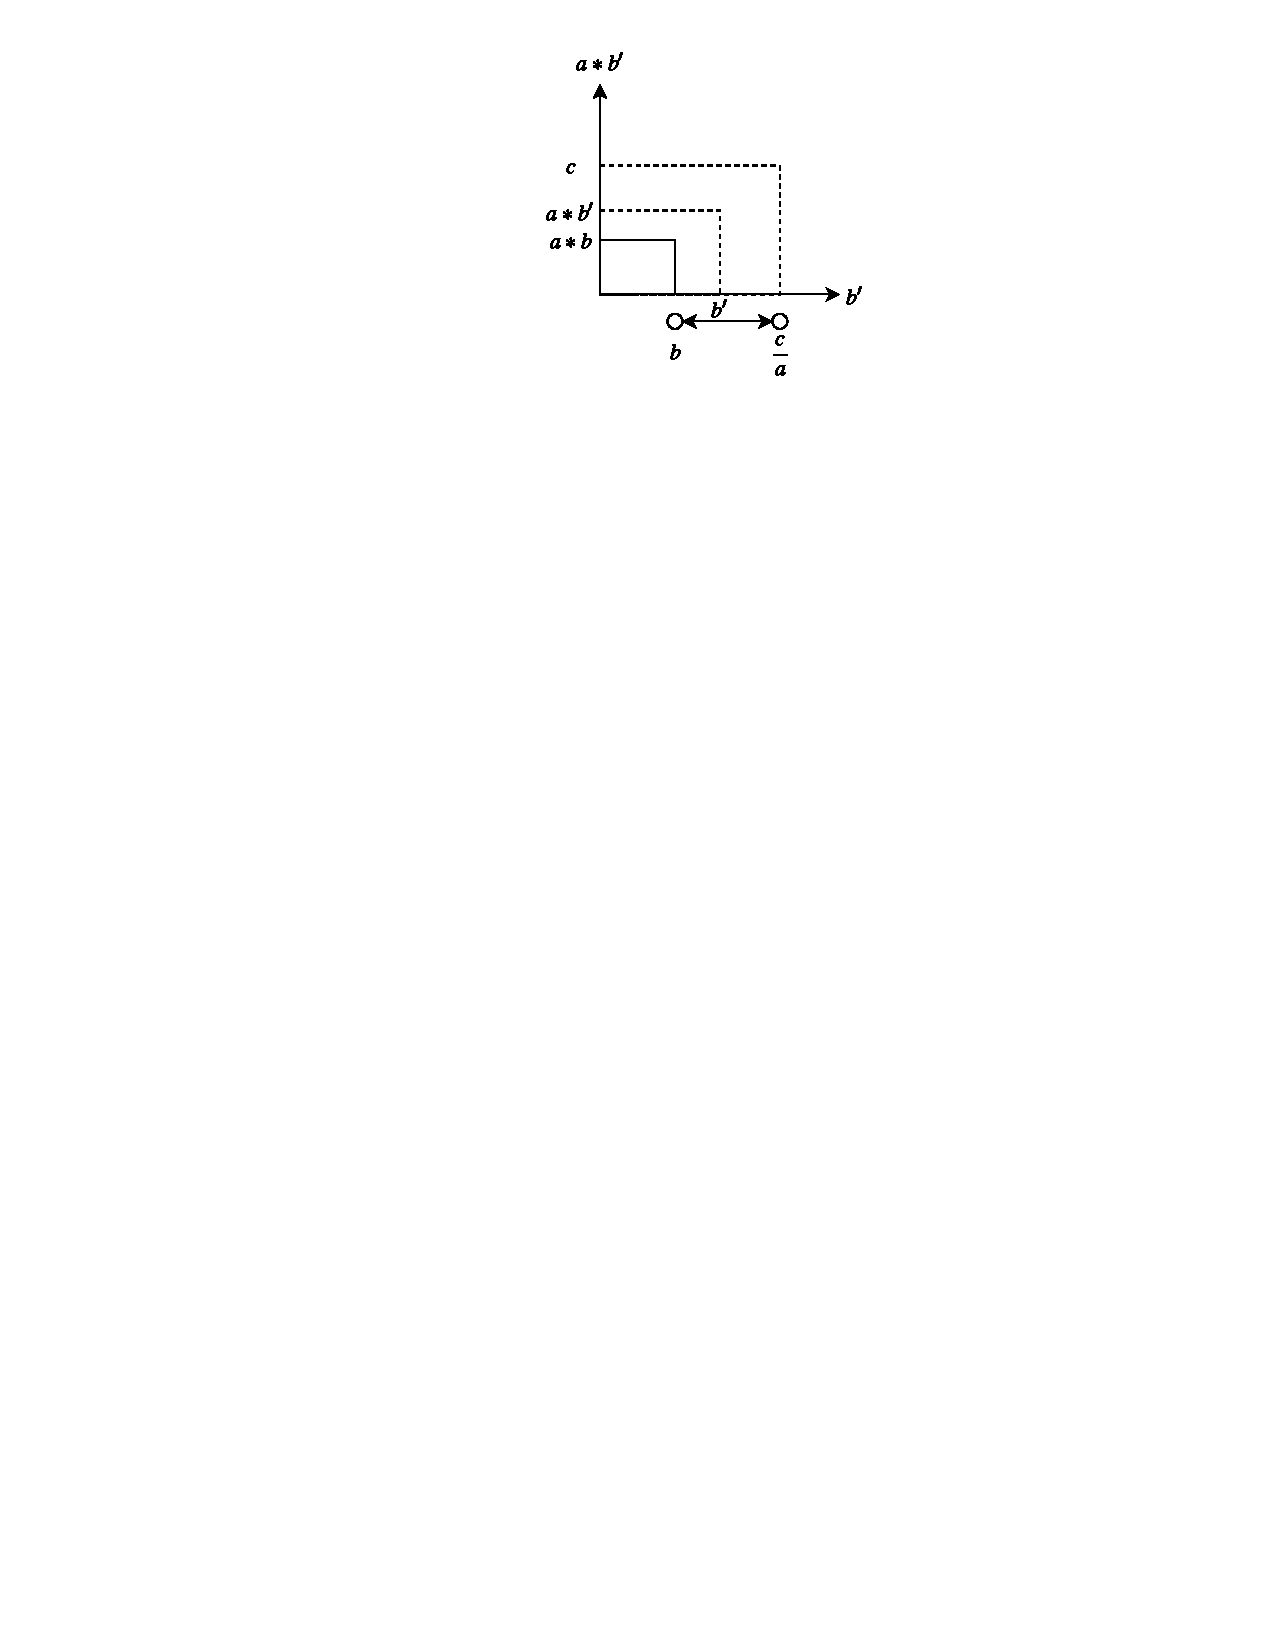
\includegraphics[scale=0.9]{../figures/ICP2_1.pdf}
    		\end{figure}
    		\centering
    		\vspace{-0.5cm}
    		Choose, $\frac{c}{a} < b^\prime \leq b$
    	\end{minipage}
    	\begin{minipage}{5cm}
    		\vspace{1cm}
    		\begin{figure}	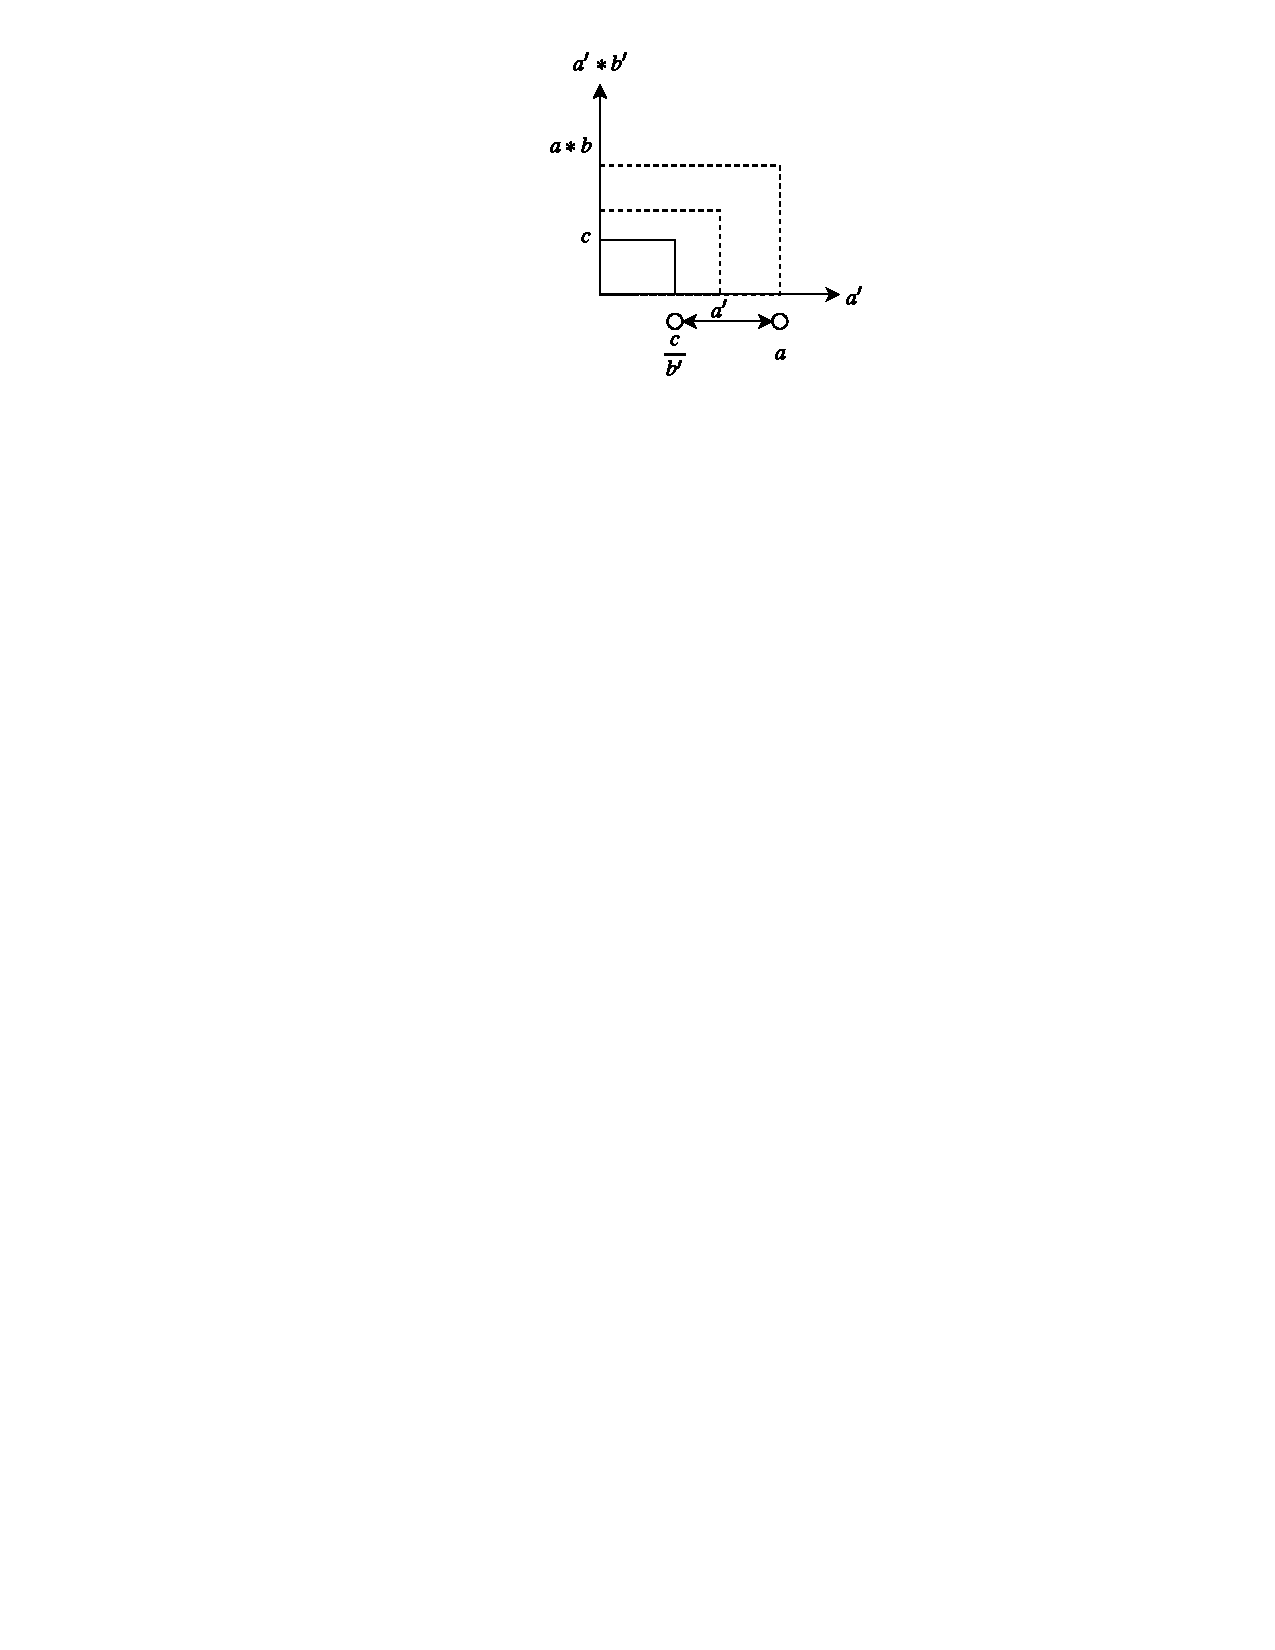
\includegraphics[scale=0.9]{../figures/ICP2_2.pdf}
    		\end{figure}
    		\centering
    		\vspace{-0.5cm}
    		Choose, $\frac{c}{b^\prime} < a^\prime \leq a$
    	\end{minipage}
    \end{overlayarea}
\end{frame}

\section{Refinement Process}
\begin{frame}{Refinement Process (Cont.)}
    \textbf{ICP (two dimensional case)}\newline So, for $c > a \ast b$ we have one axiom:
    \begin{itemize}
        \item $$(-a^\prime \leq x \leq a^\prime) \wedge (-b^\prime \leq y \leq b^\prime) \to (-c^\prime \leq z \leq c^\prime)$$
    \end{itemize}
\end{frame}

\section{Refinement Process}
\begin{frame}{Refinement Process (Cont.)}
    \textbf{ICP (one dimensional case)}
   \begin{itemize}
   \item Consider, $z = x^2$.
   \item Take the absolute values of $x, y \text{ and } z$:
$$|\mu(x)| = a, \quad  \text{ and } \quad |\mu(z)| = c$$
\end{itemize}
\end{frame}

\section{Refinement Process}
\begin{frame}{Refinement Process (Cont.)}
    \begin{itemize}
        \item We have 7 sequences of axioms. 
        \item Heuristics
        \begin{enumerate}
            \item Take the first axiom instance that is violated by the solution for the abstraction.
            \item Take all violated axiom instances.
            \item Choose axiom instances randomply from the set of all violated axiom instances.
        \end{enumerate}
    \end{itemize}
\end{frame}

\section{Example}
\begin{frame}{Example}
    \begin{itemize}
        \item \textcolor<1>{blue}{Consider the same input NRA formula $\varphi$ has the multiplication terms $t_{1} \ast s_{1}$ and $t_{2} \ast s_{2}$.}
        \item \textcolor<2>{blue}{$t_{1} \ast s_{1}$ and $t_{2} \ast s_{2}$ are abstracted by $z_{1}$ and $z_{2}$, respectively and an abstracted formula $\hat{\varphi}$ is being created.}
		\item \textcolor<3>{blue}{Let, abstract model $\hat{\mu}$ contains the assignments:
    $$\hat{\mu}[z_{1}] = 7, \quad \hat{\mu}[z_{2}] = 5$$}
    \item \textcolor<4>{blue}{Now, extend $\hat{\mu}$ and we get the following assignments:
    $$\hat{\mu}[t_{1}] = 2, \quad \hat{\mu}[s_{1}] = 3, \quad \hat{\mu}[z_{1}] = 7,$$ $$\hat{\mu}[t_{2}] = 3, \quad \hat{\mu}[s_{2}] = -4, \quad \hat{\mu}[z_{2}] = 5$$}
    \end{itemize}
\end{frame}

\section{Example}
\begin{frame}{Example (cont.)}
    \begin{itemize}
        \item \textcolor{red}{Abstract model $\hat{\mu}$:  $\hat{\mu}[t_{1}] = 2, \quad \hat{\mu}[s_{1}] = 3, \quad \hat{\mu[f_{\ast}(t_{1}, s_{1})]} = 7,$ $\hat{\mu}[t_{2}] = 3, \quad \hat{\mu}[s_{2}] = -4, \quad \hat{\mu[f_{\ast}(t_{2}, s_{2})]} = 5$}
        \item \textcolor<1>{blue}{$\hat{\mu}$ violates the third Zero constraint for $t_{2} \ast s_{2}$:
    $$((t_{2} < 0 \wedge s_{2} > 0) \vee (t_{2} > 0 \wedge s_{2} < 0)) \Leftrightarrow z_{2} < 0$$}
    \end{itemize}
\end{frame}

\section{Example}
\begin{frame}{Example (cont.)}
    \begin{itemize}
        \item \textcolor{red}{Abstract model $\hat{\mu}$:  $\hat{\mu}[t_{1}] = 2, \quad \hat{\mu}[s_{1}] = 3, \quad \hat{\mu[f_{\ast}(t_{1}, s_{1})]} = 7,$ $\hat{\mu}[t_{2}] = 3, \quad \hat{\mu}[s_{2}] = -4, \quad \hat{\mu[f_{\ast}(t_{2}, s_{2})]} = 5$}
        \item \textcolor<1>{blue}{$\hat{\mu}$ also violates the Tangent-plane constraint in the points $(2, 3)$ and $(3, -4)$}
        \item \textcolor<2>{blue}{at the point $(2, 3)$: 
    $z_{1} = 2 \ast s_{1} \quad \wedge$ \quad
    $z_{1} = 3 \ast t_{1} \quad \wedge$
    $((t_{1} > 2 \wedge s_{1} < 3) \vee (t_{1} < 2 \wedge s_{1} > 3)) \implies z_{1} < 3 \ast t_{1} + 2 \ast s_{1} - 6 \quad \wedge$
     $((t_{1} < 2 \wedge s_{1} < 3) \vee (t_{1} > 2 \wedge s_{1} > 3)) \implies z_{1} > 3 \ast t_{1} + 2 \ast s_{1} - 6$}
		\item \textcolor<3>{blue}{at the point $(3, -4)$: 
    $z_{2} = 3 \ast s_{2} \quad \wedge$ \quad
    $z_{2} = -4 \ast t_{2} \quad \wedge$
    $((t_{2} > 3 \wedge s_{2} < -4) \vee (t_{2} < 3 \wedge s_{2} > -4)) \implies z_{2} < -4 \ast t_{2} + 3 \ast s_{2} + 12 \quad \wedge$
     $((t_{2} < 3 \wedge s_{2} < -4) \vee (t_{2} > 3 \wedge s_{2} > -4)) \implies z_{2} > -4 \ast t_{2} + 3 \ast s_{2} + 12$}
    \end{itemize}
\end{frame}

\section{Experimental Result}
\begin{frame}{Experimental Result}
\begin{figure}
    \caption{Number of solved instances for our solvers without preprocessing (WoP)}
    \centering
    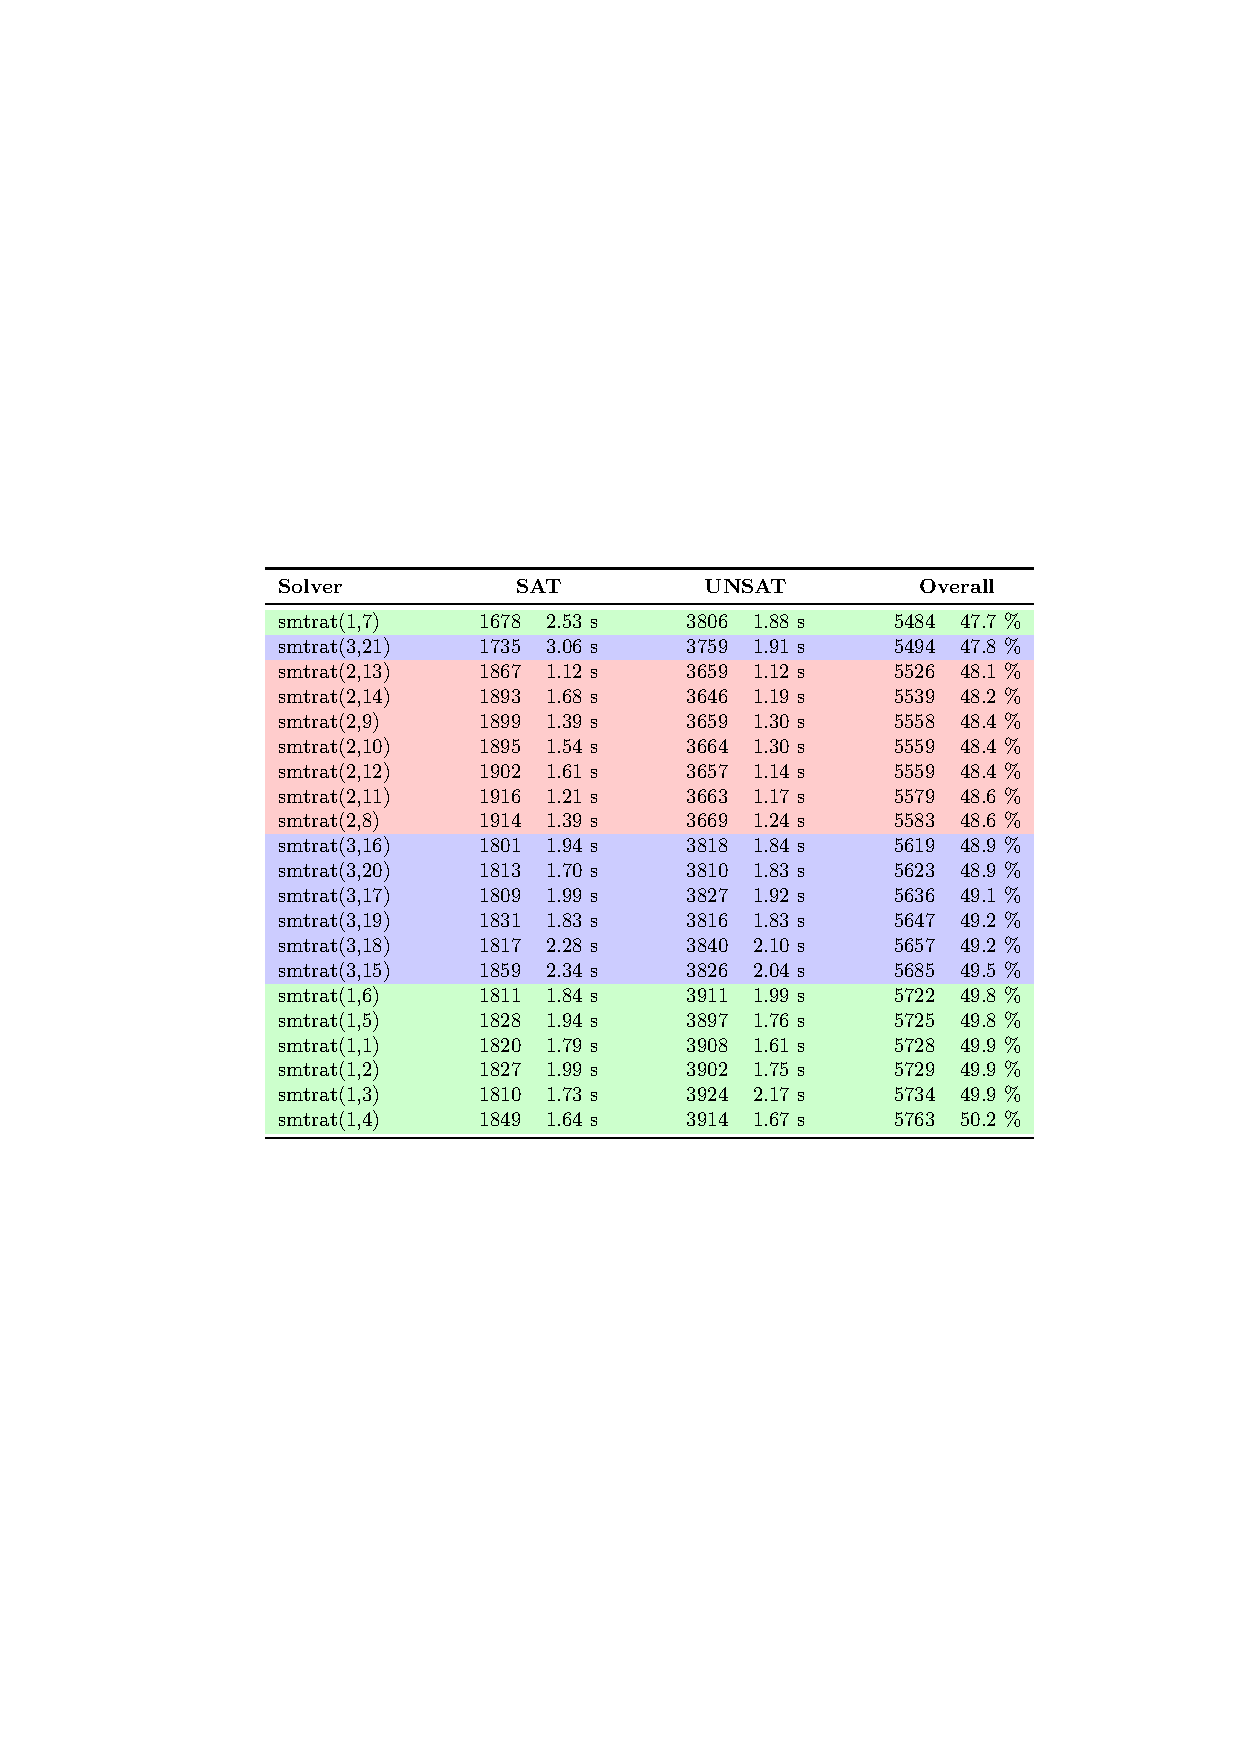
\includegraphics[scale=0.7]{../figures/OurSolver.pdf}
\end{figure}
\end{frame}

\section{Experimental Result}
\begin{frame}{Experimental Result}
\begin{figure}
    \caption{Comparison of smtrat4 with mathsat and z3}
    \centering
    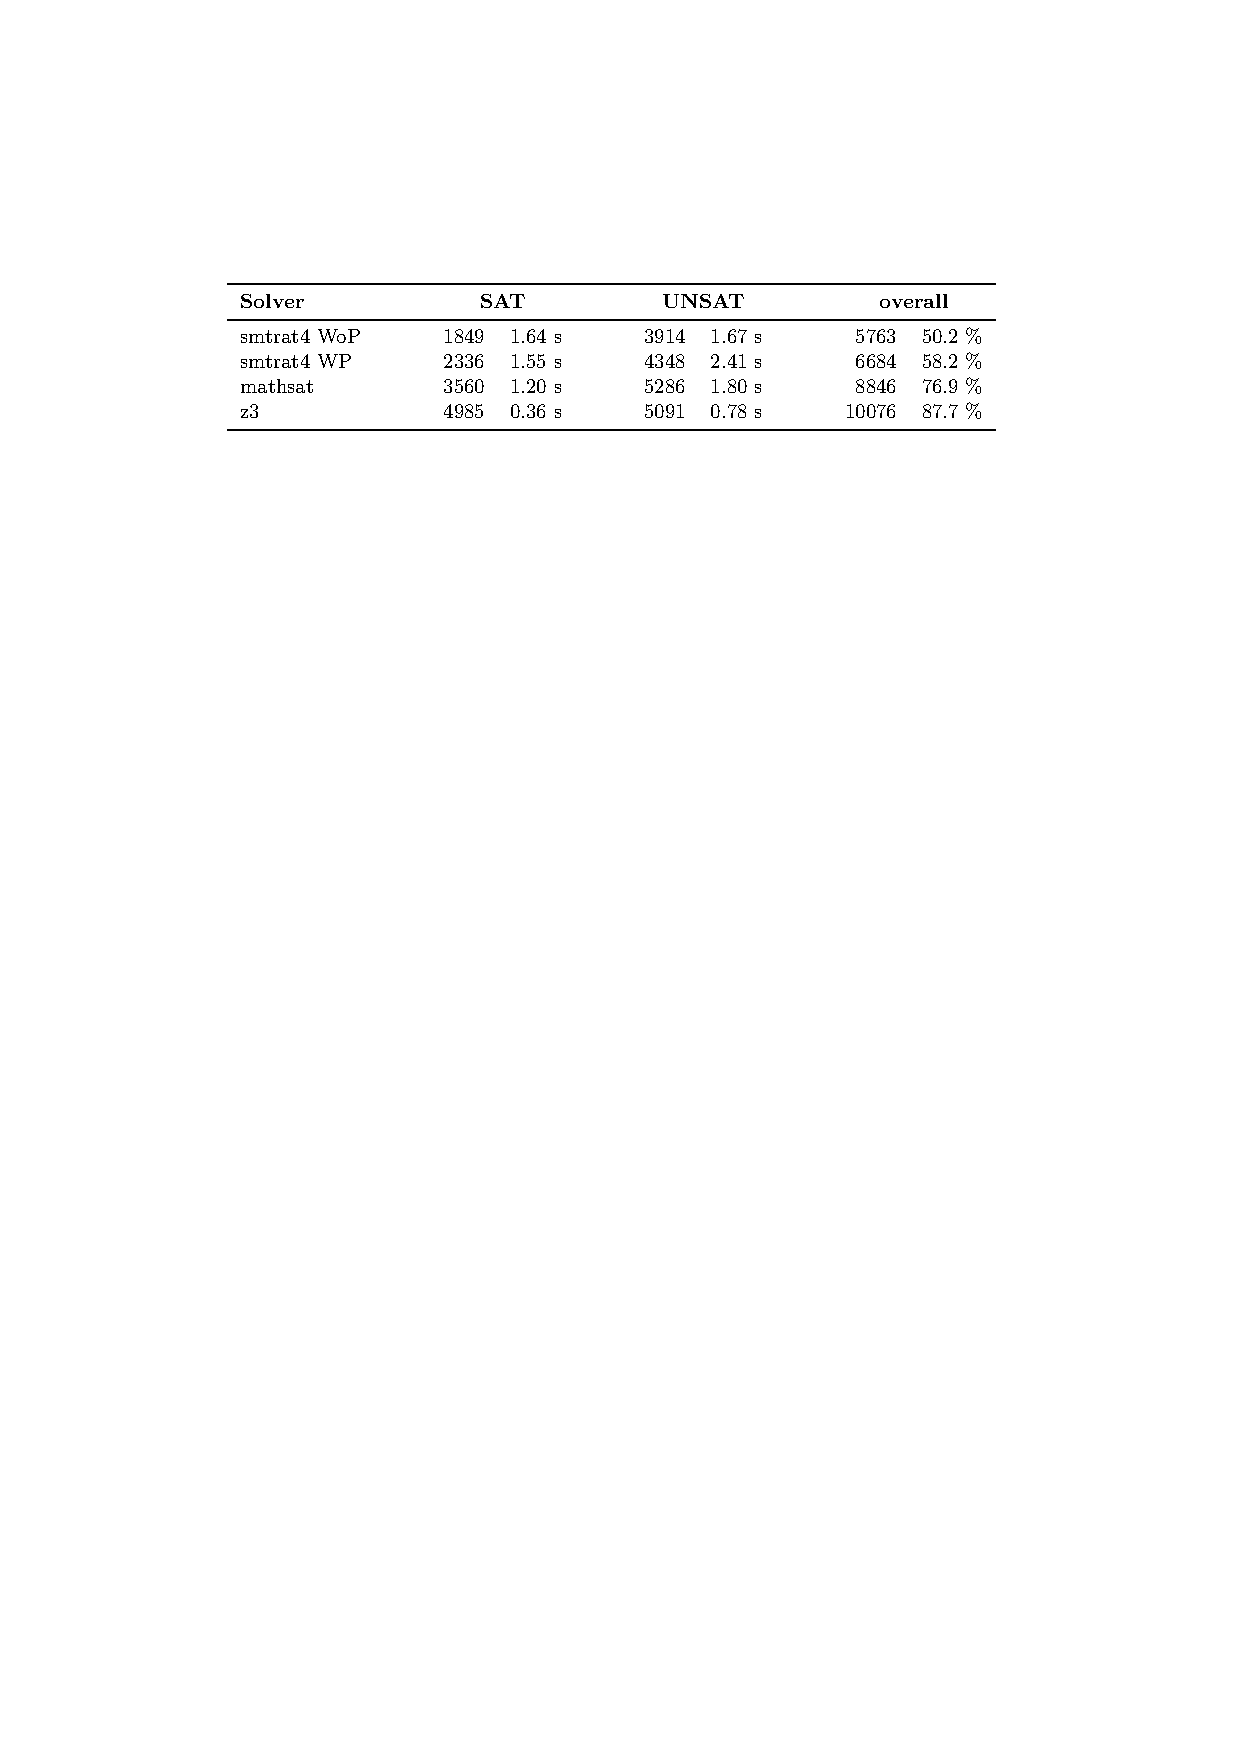
\includegraphics[scale=0.9]{../figures/ComparisonWithOthers.pdf}
\end{figure}
\end{frame}

\section{Experimental Result}
\begin{frame}{Experimental Result}
\begin{figure}
    \caption{Survival plots for smtrat4 WoP, smtrat WP, mathsat and z3}
    \centering
    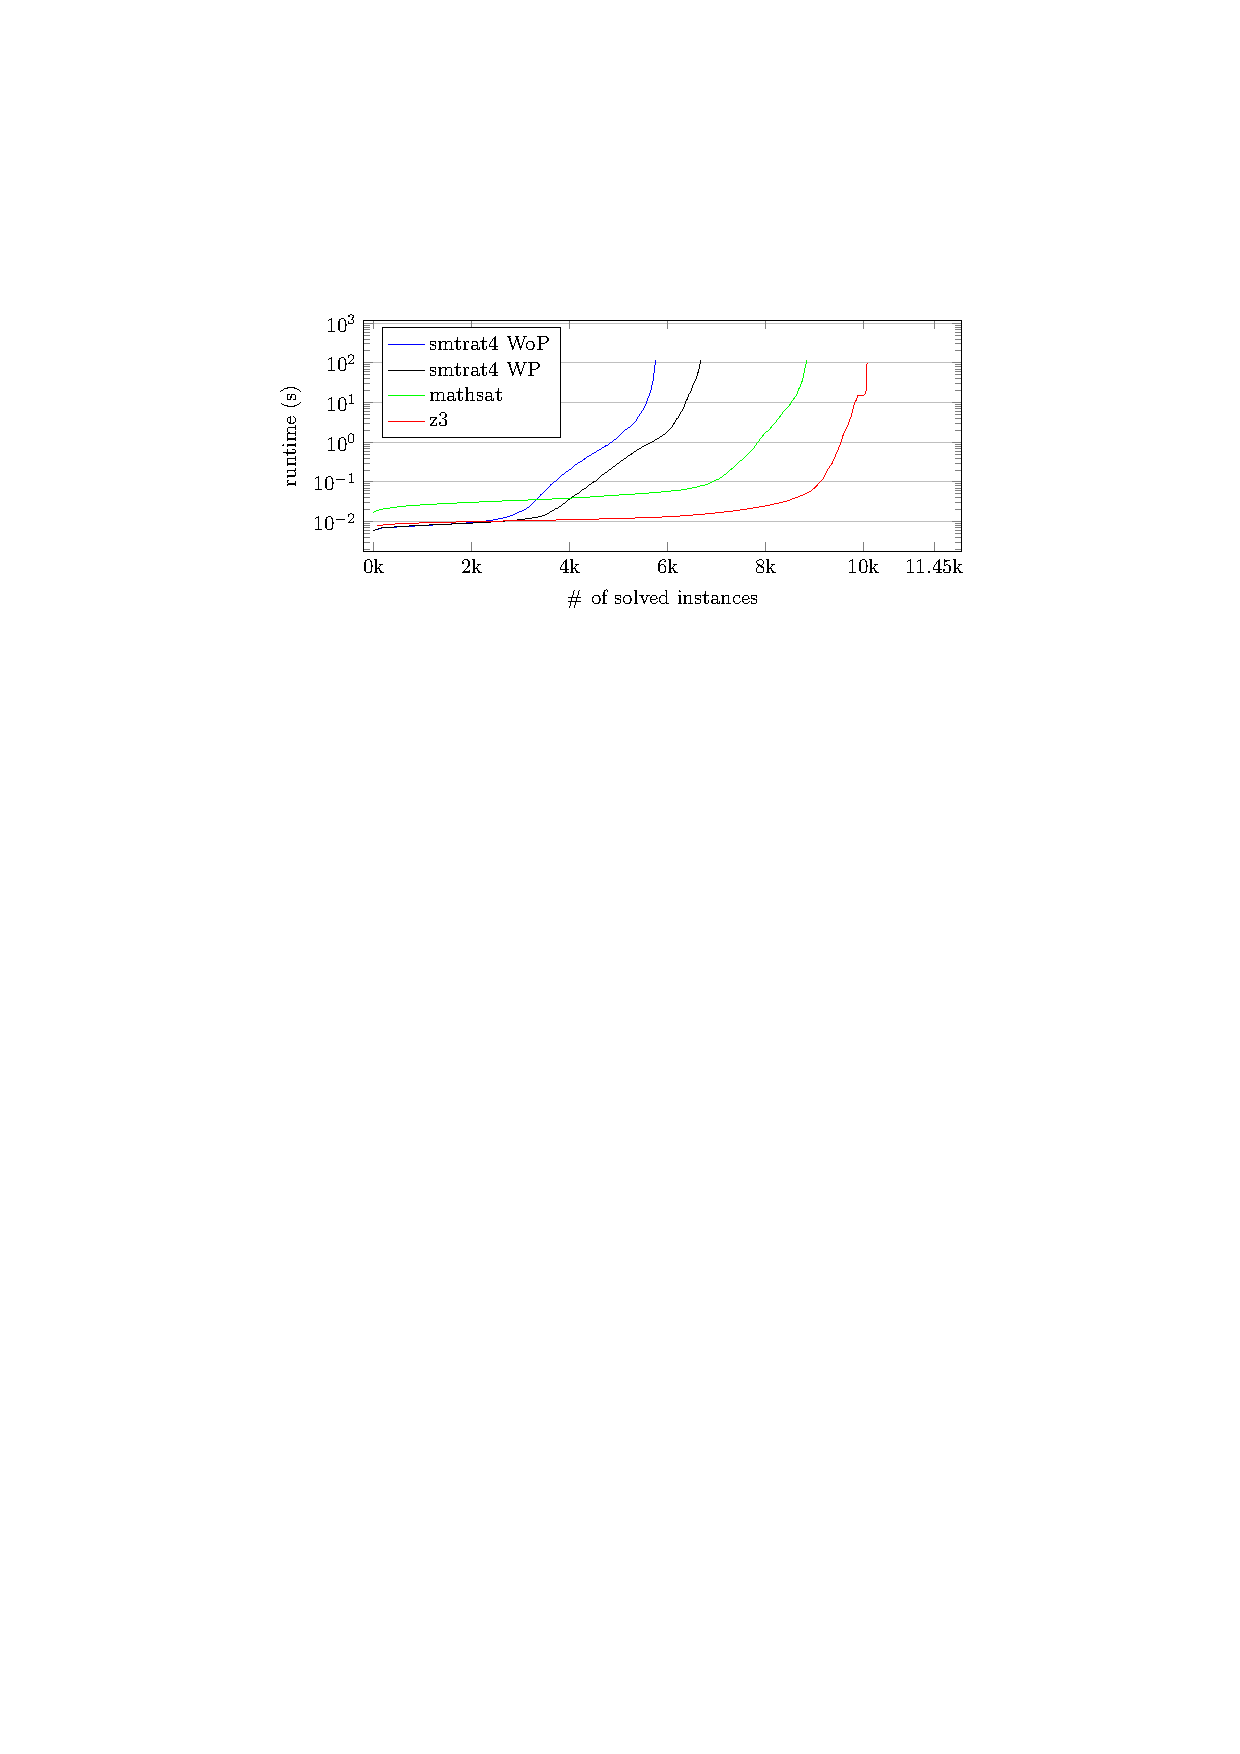
\includegraphics[scale=1]{../figures/solved_instances.pdf}
\end{figure}
\end{frame}

\section{Experimental Result}
\begin{frame}{Experimental Result}
\begin{figure}[!ht]
    \centering
    \caption{Scatter plot for smtrat4 WP and mathsat}
    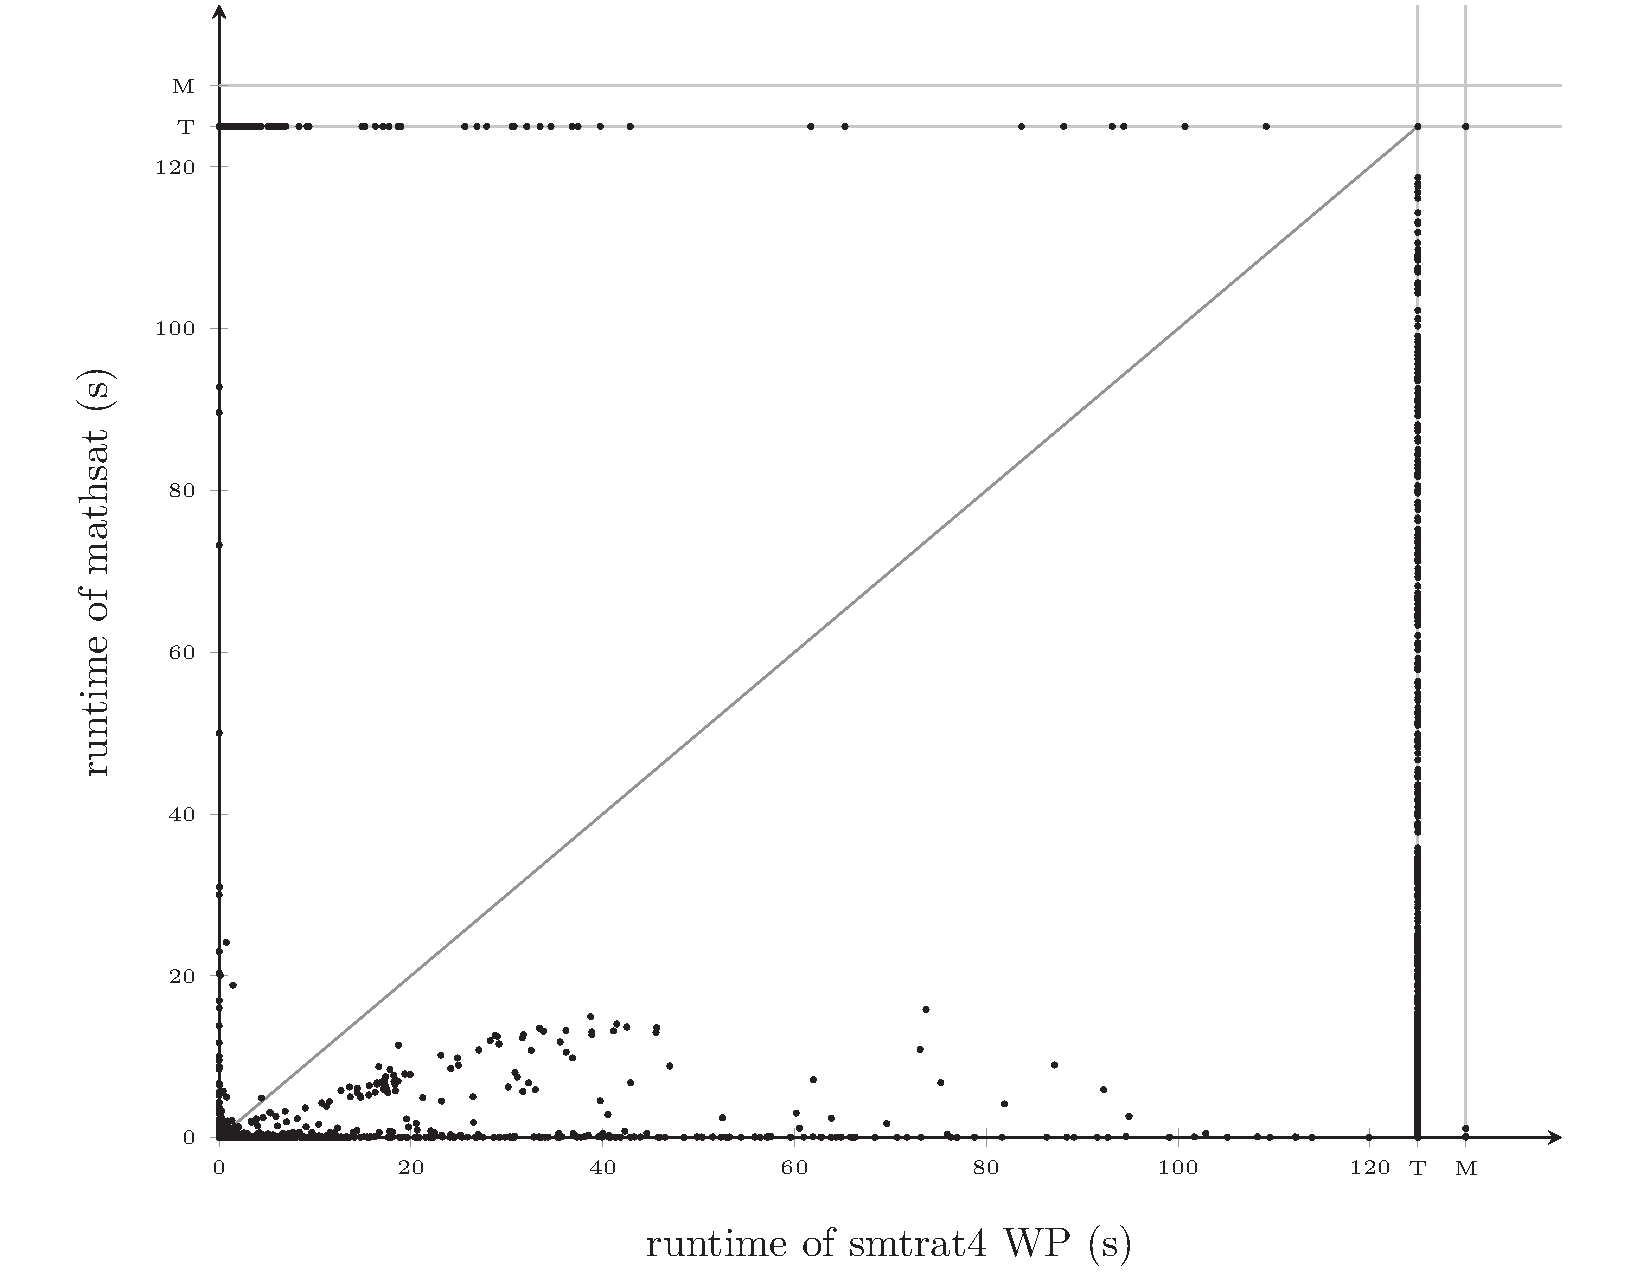
\includegraphics[width=.75\linewidth]{../figures/scatter-smtrat_4_preprocessing-mathsat.pdf}
\end{figure}
\end{frame}

\section{Experimental Result}
\begin{frame}{Experimental Result}
\begin{figure}[!ht]
    \centering
    \caption{Scatter plot for smtrat4 WP and z3}
    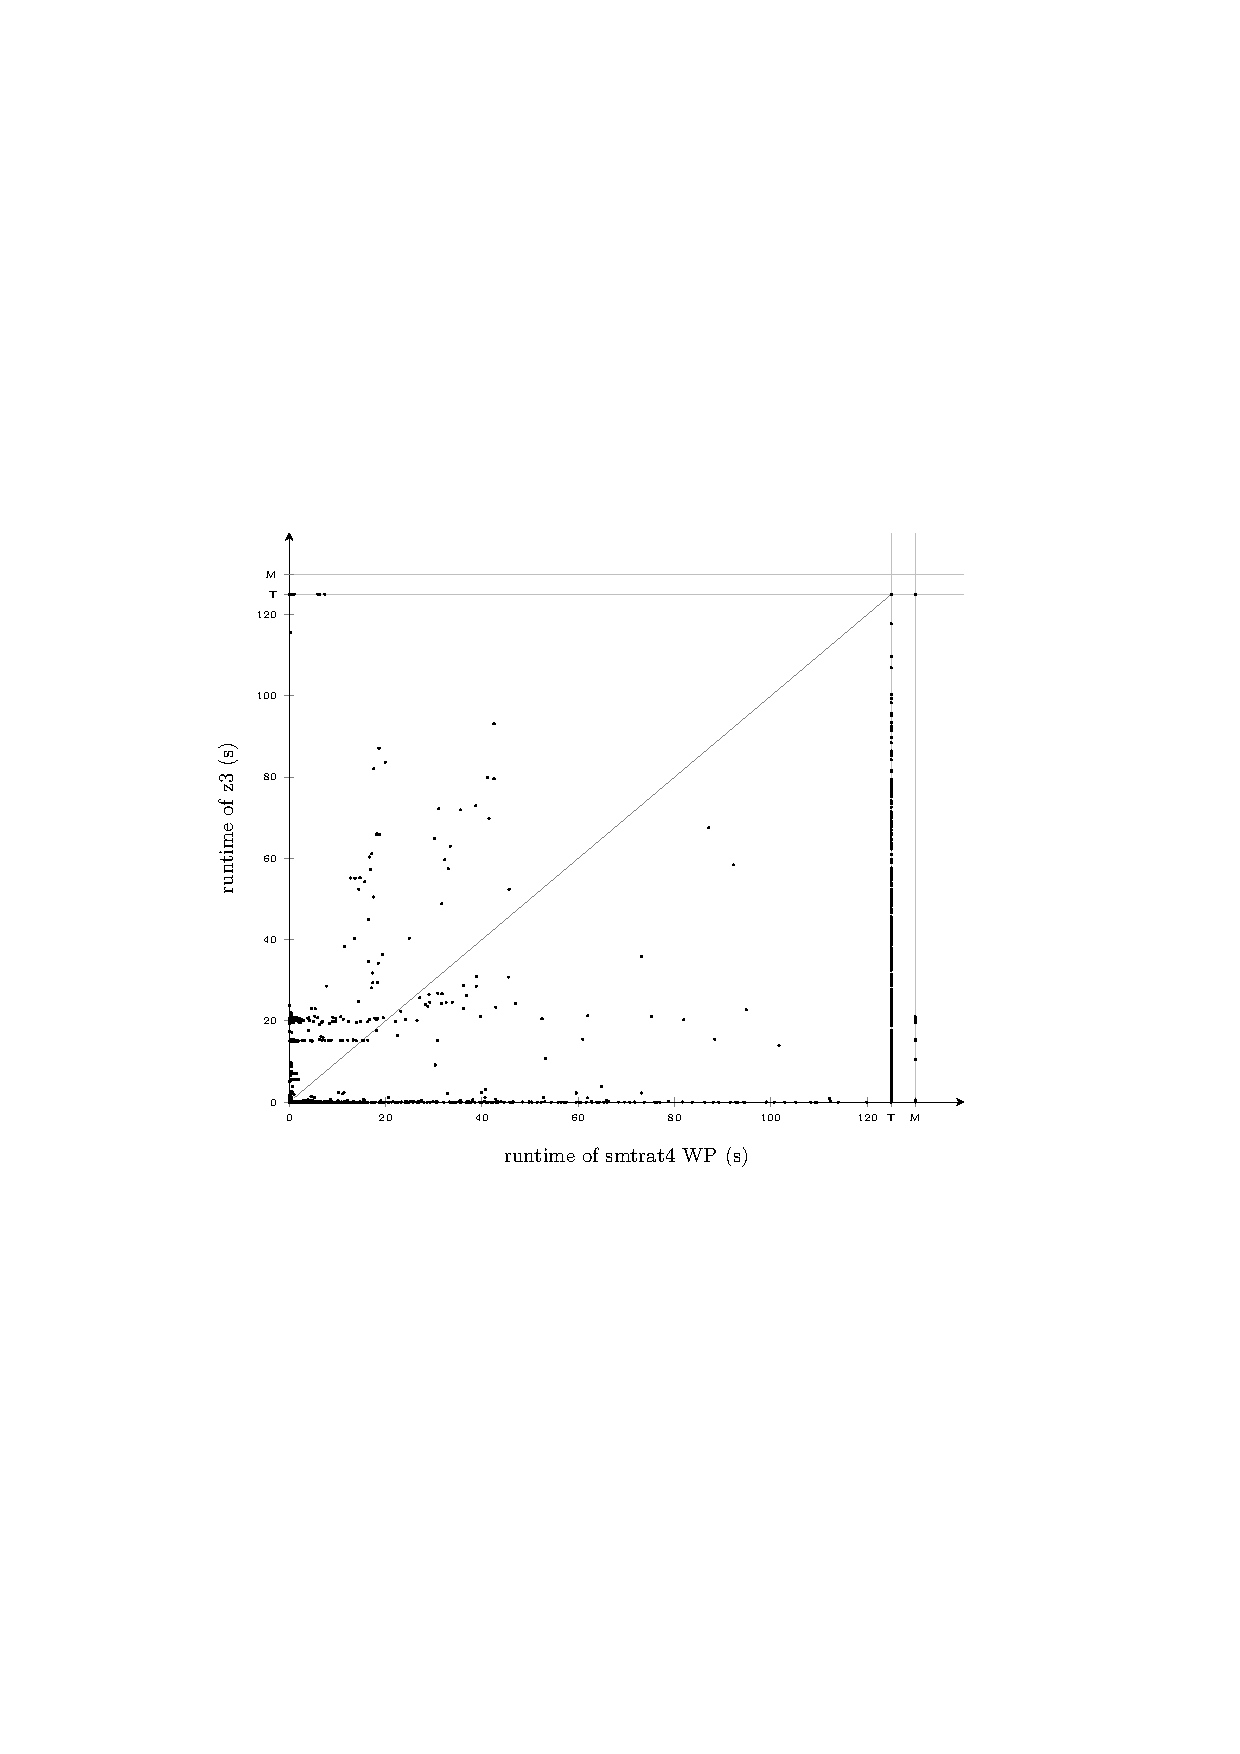
\includegraphics[width=.75\linewidth]{../figures/scatter-smtrat_4_preprocessing-z3.pdf}
\end{figure}
\end{frame}

\section{Experimental Result}
\begin{frame}{Experimental Result}
\begin{figure}[!ht]
    \centering
    \caption{Summary of smrat4, other additional smtrat solvers, mathsat and z3}
    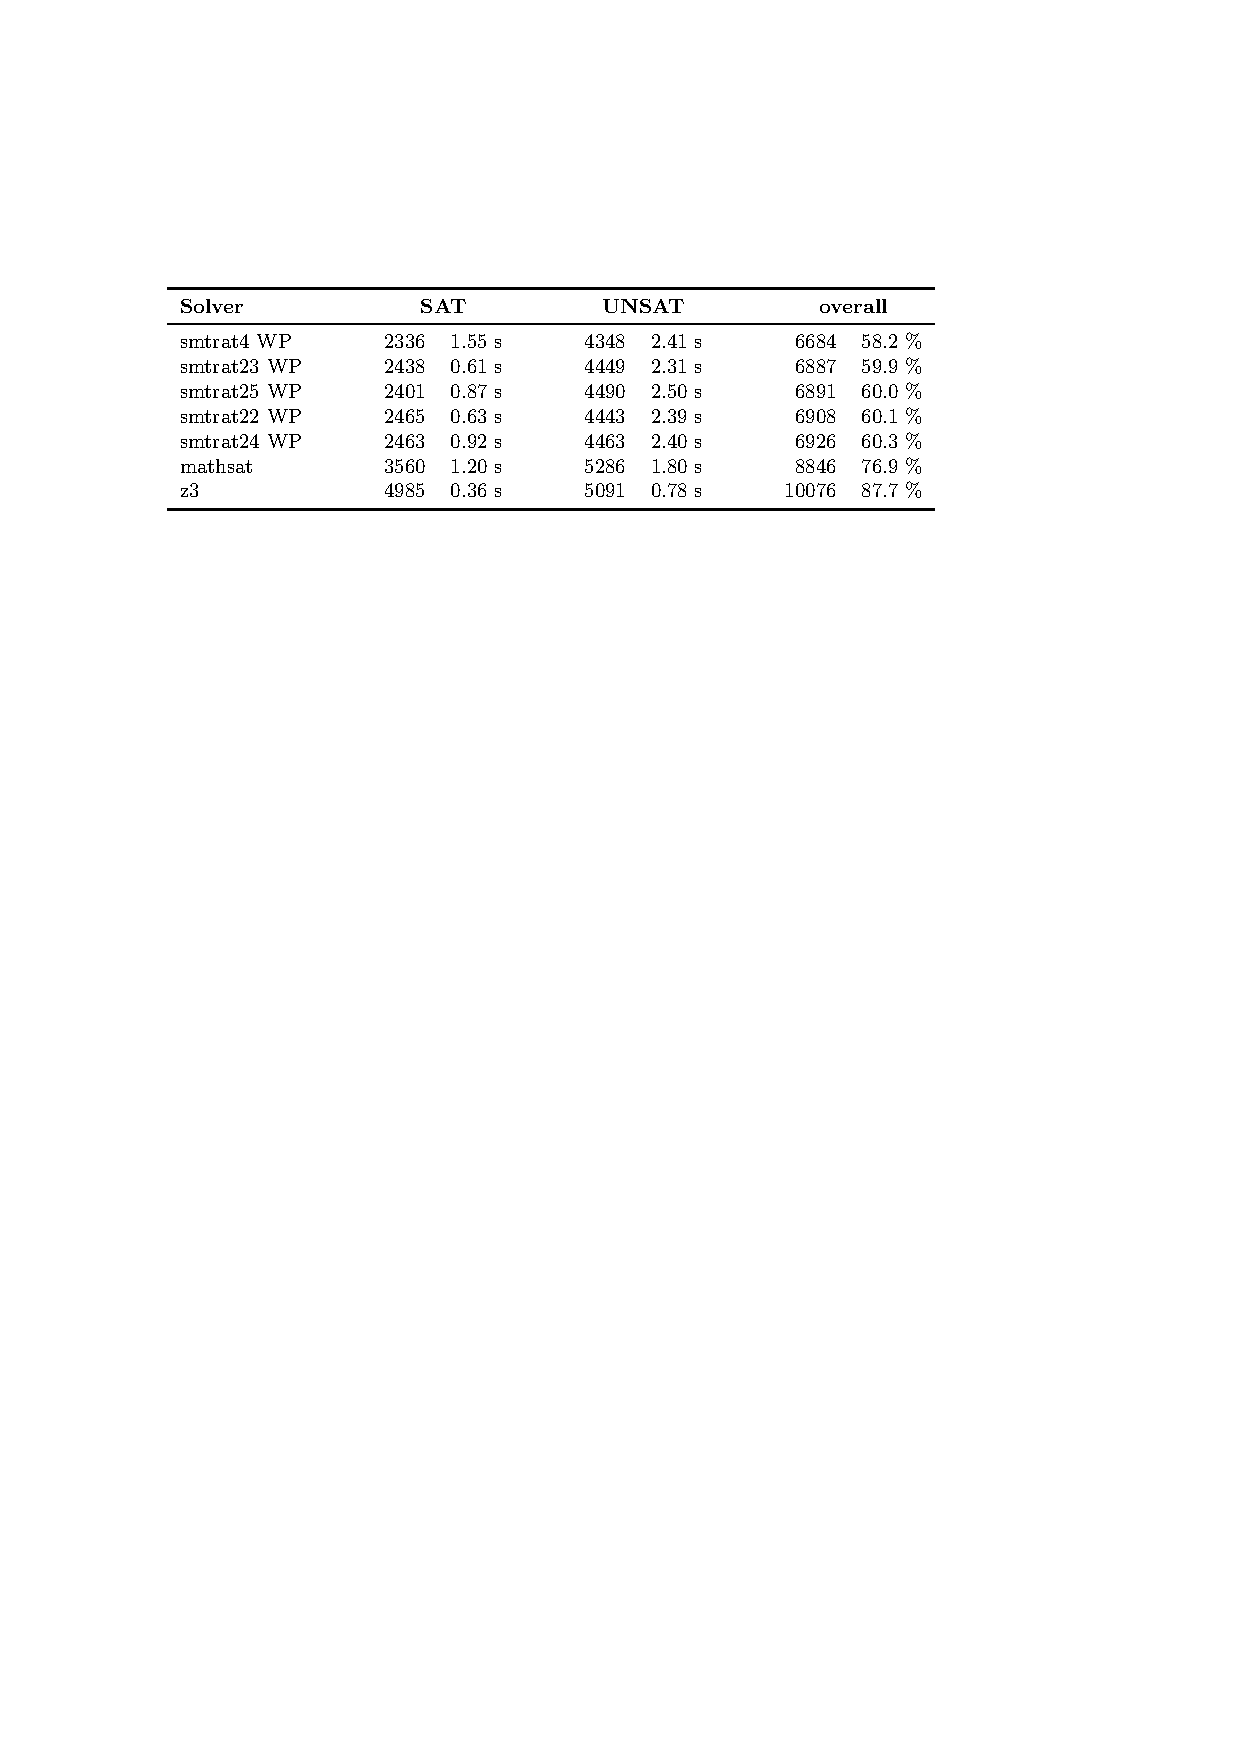
\includegraphics[width=1\linewidth]{../figures/summarySolvers.pdf}
\end{figure}
\end{frame}

\section{Experimental Result}
\begin{frame}{Experimental Result}
\end{frame}

\section{Experimental Result}
\begin{frame}{Experimental Result}
\end{frame}

\section{Future Work}
\begin{frame}{Future Work}
    \begin{itemize}
        \item Currently, we can exclude only boxes by ICP. 
        However, it is also possible to exclude the convexes of different shapes based on templates.
        That means we can try other forms of areas which we want to exclude and then derive axioms for them.
        \item Repair the abstract model.
    \end{itemize} 
\end{frame}

\section{Conclusion}
\begin{frame}{Conclusion}
    \begin{itemize}
        \item We have integrated this method as a module in SMT-RAT.
        \item The performance is satisfactory as this module is a prototype.
        \item We are expecting a significant enhancement of the performance once the mentioned future works will be integrating with the module.
    \end{itemize}
\end{frame}

\end{document}

